%----------------------------------------------------------------------------------------
%	PACKAGES AND OTHER DOCUMENT CONFIGURATIONS
%----------------------------------------------------------------------------------------

\documentclass[12pt]{article}
\usepackage{polski}
\usepackage[polish]{babel}
\usepackage[utf8]{inputenc}
\usepackage{datetime}
\usepackage{graphicx}
\usepackage{tikz}
\usepackage{amsmath}
\usepackage{multirow}
\usepackage{tabularx}
\usepackage{geometry}
\usepackage{subcaption}
\usepackage{epstopdf}
\usepackage{hyperref}
\usepackage{indentfirst}

\geometry{
 	a4paper, 
 	left    = 20mm,
 	right	  = 20mm,
 	top     = 20mm,
 	bottom  = 20mm,
}
 
%----------------------------------------------------------------------------------------
 
%----------------------------------------------------------------------------------------
% DATES
%----------------------------------------------------------------------------------------

\renewcommand{\dateseparator}{.}
\newdate{exercise_date}{15}{12}{2016}


% dodatkowe typy kolumn tabel

% flush left fixed width:
\newcolumntype{L}[1]{>{\raggedright\arraybackslash}p{#1}}

% center fixed width:
\newcolumntype{C}[1]{>{\centering\arraybackslash}p{#1}}

% flush right fixed width:
\newcolumntype{R}[1]{>{\raggedleft\arraybackslash}p{#1}}

%----------------------------------------------------------------------------------------

%----------------------------------------------------------------------------------------
% TIKZ PACKAGES
%----------------------------------------------------------------------------------------

\usetikzlibrary{arrows}

%----------------------------------------------------------------------------------------

\begin{document}
 
\begin{titlepage}

\newcommand{\HRule}{\rule{\linewidth}{0.5mm}}
% Defines a new command for the horizontal lines, change thickness here

\center
% Center everything on the page
 
%----------------------------------------------------------------------------------------
%	LOGO SECTION
%----------------------------------------------------------------------------------------


\includegraphics[width=6cm]{./img/logo.png}\\[1cm]
% Include a department/university logo - this will require the graphicx package
 
%----------------------------------------------------------------------------------------
 
%----------------------------------------------------------------------------------------
%	HEADING SECTIONS
%----------------------------------------------------------------------------------------

\textsc{\LARGE Akademia Górniczo-Hutnicza \\[0.2cm]
im. Stanisława Staszica w Krakowie}\\[1.5cm]
% Name of your university/college

\textsc{\Large Elektroniczne systemy diagnostyki medycznej i terapii}\\[0.5cm]
% Major heading such as course name

%----------------------------------------------------------------------------------------
%	TITLE SECTION
%----------------------------------------------------------------------------------------

\HRule \\[0.5cm]
{ \huge \bfseries Klasyfikacja pulsu - Naiwny Bayes}\\[0.3cm]
% Title of your document
\HRule \\[1.5cm]

\flushright
\Large \emph{Autorzy:}\\
Piotr \textsc{Janus}\\[0.1cm]  % Your name
Kamil \textsc{Piszczek}\\[3cm]        % Your name
% Authors

%----------------------------------------------------------------------------------------
%	DATE SECTION
%----------------------------------------------------------------------------------------
% Data wykonania ćwiczenia: \\
%{\large \displaydate{exercise_date}}\\[1cm]


\vfill % Fill the rest of the page with whitespace

\end{titlepage}
\section{Wstęp}
\label{sec_wstep}

Naiwny klasyfikator Bayesa jest prostym klasyfikatorem probabilistycznym opartym na twierdzeniu Bayesa. Jest nazywany naiwnym ze względu na przyjęte założenie, mówiące, że poszczególne cechy są wzajemnie niezależne. Pomimo tak dużego uproszczenia, klasyfikator wypada niespodziewanie dobrze w wielu rzeczywistych problemach. Jego dużą zaletą jest dobra skalowalność, operuje on jedynie na jawnych wzorach w przeciwieństwie do innych metod wykorzystujących podejście iteracyjne.

Jednym z zastosowań klasyfikatora jest diagnozowanie wad i dysfunkcji serca na podstawie sygnału EKG, a dokładniej występującego w nim zespołu QRS. Jest to zespół opisujący pobudzenie mięśni serca. Uproszczony przebieg EKG z zespołem QRS został umieszczony na rysunku \ref{fig_qrs}.

\begin{figure}[!htb]
  \begin{center}
    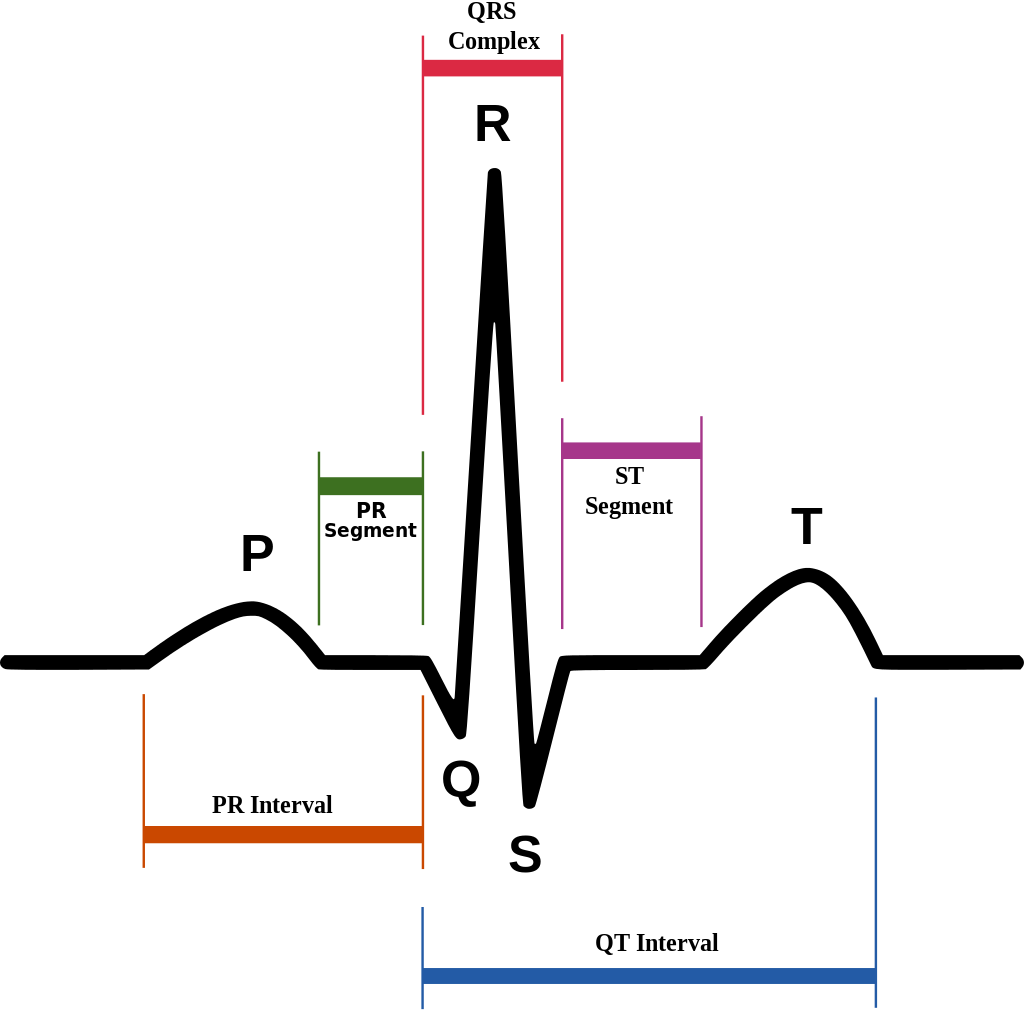
\includegraphics[scale = 0.25]
    {img/qrs.png}
  \end{center}
  \caption{Uproszczony zespół QRS -- źródło \cite{bibWikipedia}}
  \label{fig_qrs}
\end{figure}

W celu dokonania klasyfikacje konieczne jest zdefiniowanie wskaźników opisujących QRS. Na podstawie rysunku \ref{fig_qrs} możemy wyróżnić następujący cechy:

	\begin{itemize}
	\item{Wartość szczytowa załamka R i moment jej wystąpienie} 
	\item{Odstęp pomiędzy wcześniejszym a obecnie analizowanym załamkiem R}
	\item{Odstęp pomiędzy aktualnie analizowanym i kolejnym załamkiem R}
	\item{Początek/koniec oraz początkowa/końcowa wartość załamka P}
	\item{Wartość szczytowa załamka P i moment jej wystąpienia}
	\item{Początek/koniec i wartość początkowa/końcowa całego zespołu QRS}
	\item{Wartość szczytowa załamka T i moment jego wystąpienia}
	\item{Koniec i wartość końcowa załamka T}
	\end{itemize}
\section{Algorytm}
\label{sec_algorytm}

\subsection{Założenia}
\label{subsec_zalozenia}

Idee metody Naiwnego Bayesa można łatwo wyjaśnić na prostym przykładzie, precyzyjny opis matematyczny został zamieszczony w rozdziale \ref{sec_opis_mat}. Na rysunku \ref{fig_bayes_przyklad} przedstawiony został zbiór punktów, podzielony na dwie klasy (czerwone i zielone). Zadaniem klasyfikatora jest przydzielenie nowego obiektu do jednej z tych klas. W tym przypadku klasyfikacja będzie dokonana na podstawie położenia i elementów znajdujących się w sąsiedztwie nowo dodanego obiektu. Podany zbiór punktów, pełni w tym przypadku rolę zbioru uczącego.

\begin{figure}[!htb]
  \begin{center}
    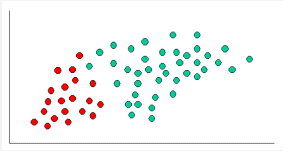
\includegraphics[scale = 1]
    {img/bayes_przyklad.png}
  \end{center}
  \caption{Prosty przykład - zbiór punktów (źródło \ref{})}
  \label{fig_bayes_przyklad}
\end{figure}

\subsection{Klasyfikacja}
\label{subsec_klasyfikacja}

W omawianym przykładzie możemy zauważyć, że obiektów zielonych jest dwa razy więcej niż czerwonych. W związku z tym możemy założyć ''z góry'', że nowy obiekt ma dwa razy większe prawdopodobieństwo bycia zielonym niż czerwonym. Obliczone w ten sposób prawdopodobieństwo nazywane jest prawdopodobieństwem \textit{a priori}. 

Wszystkich obiektów jest 60 w czym 40 zielonych i 20 czerwonych. Prawdopodobieństwo \textit{a priori} wylicza się jako iloraz liczby obiektów danego koloru do liczby wszystkich obiektów. Następnie przystępujemy do kolejnego etapu klasyfikacji, przyjmijmy pewne sąsiedztwo nowego punktu (rysunek \ref{fig_bayes_przyklad2}). Możemy założyć, że im więcej obiektów danego koloru w otoczeniu nowego obiektu, tym bardziej prawdopodobne, że jest on tego koloru. Wyznaczone w ten sposób prawdopodobieństwo nazywane jest szansą, oblicza się je jako stosunek liczby obiektów danego koloru w sąsiedztwie, do całkowitej liczby obiektów tego koloru.

\begin{figure}[!htb]
  \begin{center}
    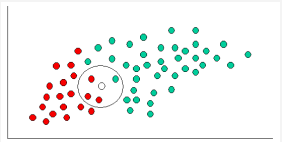
\includegraphics[scale = 1]
    {img/bayes_przyklad_2.png}
  \end{center}
  \caption{Prosty przykład - sąsiedztwo (źródło \ref{})}
  \label{fig_bayes_przyklad2}
\end{figure}

Mając dane prawdopodobieństwo \textit{a priori} oraz szansę, możemy przystąpić do ostatniego etapu klasyfikacji. Końcowe prawdopodobieństwo czy nowy obiekt należy do danej klasy (jest danego koloru) obliczane jest jako iloczyn dwóch wyznaczonych wcześniej prawdopodobieństw. Zostaje on oczywiście przypisany do klasy o większym prawdopodobieństwie.


\subsection{Wykorzystanie w detekcji pulsu}
\label{subsec_bayes_detekcja_pulsu}

Omówiony w poprzednich punktach przykład, był bardzo uproszczony i miał na celu jedynie pokazać idee klasyfikatora. Klasyfikacja zespołu QRS jest problemem wielowymiarowym (dokładnie 18 wymiarowym, gdyż jest to rozmiar wektora cech). W takim przypadku nieco inaczej oblicza ''szansa''. Obliczane jest osobno prawdopodobieństwo przynależności do danej klasy na podstawie każdego elementu z wektora cech. Ostatecznie pod uwagę brany jest iloczyn wszystkich prawdopodobieństw.

Kolejnym zagadnieniem jest sposób obliczania prawdopodobieństwa na podstawie cechy. W przypadku niniejszego projektu wykorzystywany jest w tym celu rozkład normalny (rozdział \ref{sec_rozklady}). Dla każdej klasy, poszczególne cechy mają przypisaną wartość średnią i odchylenie standardowe. Są one obliczane na podstawie zbioru uczącego w trakcie procesu uczenia.

\subsection{Zbiór testowy i uczący}
\label{subsec_test_ucz}


\section{Opis matematyczny}
\label{sec_opis_mat}

\subsection{Twierdzenie Bayesa}
\label{subsec_tw_bayesa}
Twierdzenie w teorii prawdopodobieństwa określające zależność między prawdopodobieństwem warunkowym wystąpienia zdarzeń $A|B$ i $B|A$. Przyjmijmy zbiór zdarzeń $X$, w którym zdarzenia $B_i \in X$, $P(B_i)>0$ ${(i=1,2, \dots , n)}$ tworzą układ zupełny (iloczyn każdych dwóch zdarzeń jest zdarzeniem niemożliwym, natomiast suma wszystkich zdarzeń jest zdarzeniem pewnym). Wówczas dla dowolnego $A \in X$ zachodzi następująca zależność:

	\begin{equation}
	\label{eq_tw_bayesa_1}
		P(B_i | A) = \frac{P(A | B_i) P(B_i)}{P(A)}
	\end{equation}

Wykorzystując dodatkowo wzór na prawdopodobieństwo całkowite, powyższa zależność może zostać przekształcona do następującej postaci:

	\begin{equation}
	\label{eq_tw_bayesa_2}
		P(B_i | A) = \frac{P(A | B_i) P(B_i)}{\sum_{k=1}^{n} P(A | B_k)P(B_k)}
	\end{equation}


\subsection{Model probabilistyczny}
\label{subsec_model}

Zdefiniujmy k-elementowy zbiór klas $C = {\{C_1, C_2, \dots, C_k\}}$ oraz dane do klasyfikacji opisane jako wektor ${x = \{x_1, x_2, \dots, x_n\}}$ zawierający $n$ niezależnych cech. Prawdopodobieństwo przynależności do danej klasy może zostać zapisane z wykorzystaniem twierdzenia Bayesa (rozdział \ref{subsec_tw_bayesa}):

	\begin{equation}
	\label{eq_p_ck_x}
		P(C_i | x) = \frac{P(x | C_i) P(C_i)}{P(x)}
	\end{equation}

Prawdopodobieństwo $P(x)$ występujące w mianowniku wzoru (\ref{eq_p_ck_x}) nie zależy od $C$ i jest stałe, licznik może natomiast zostać przekształcony poprzez wykorzystanie definicji prawdopodobieństwa warunkowego:

	\begin{equation}
	\label{eq_p_numerator1}
		P(x_1, \dots , x_n | C_i)P(C_i) = P(x_1, \dots, x_n, C_i)
	\end{equation}

	\begin{equation}
	\label{eq_p_numerator2}
		P(x_1, \dots, x_n, C_i) = P(x_1 | x_2 , \dots , x_n, C_i)P(x_2 | x_3, \dots , x_n, 	C_i) \dots P(x_{n-1} | x_n, C_i)P(x_n | C_i)P(C_i)
	\end{equation}
	
Wykorzystując przyjęte na początku założenie, że cechy ${x_1, \dots, x_n}$ są niezależne można wyprowadzić następującą zależność:

	\begin{equation}
	\label{eq_p_numerator_simp1}
		P(x_j | x_{j+1}, \dots , x_n, C_i) = P(x_j | C_i) \quad dla \quad j = \{1, 2, \dots, n-1\}
	\end{equation}

Podstawiając (\ref{eq_p_numerator_simp1}) do równania (\ref{eq_p_numerator2}) otrzymujemy:
	
	\begin{equation}
	\label{eq_p_numerator_simp2}
		P(x_1, \dots, x_n, C_i) = P(C_i) \prod_{j = 1}^n P(x_j | C_i)
	\end{equation}

Ostatecznie wzór (\ref{eq_p_ck_x}) można zapisać w postaci:

	\begin{equation}
	\label{eq_p_ck_x_simp}
		P(C_i | x) = \frac{P(C_i) \prod_{j = 1}^n P(x_j | C_i)}{P(x)}
	\end{equation}


\subsection{Rozkłady prawdopodobieństwa}
\label{sec_rozklady}

\subsubsection{Rozkład normalny}
\label{subsec_gauss}

	\begin{equation}
	\label{eq_gauss}
	p(x_i | C_j) = \frac{1}{\sigma \sqrt{2 \pi}}\exp\bigg(\frac{-(x-\mu_{ij})^2}{2\sigma_{ij}^2)}\bigg), \quad
	-\infty < x < \infty, \; -\infty < \mu_{ij} < \infty, \; \sigma_{ij}  > 0
	\end{equation}


\subsubsection{Rozkład lognormalny}
\label{subsec_lognorm}

	\begin{equation}
	\label{eq_lognorm}
	p(x_i | C_j) = \frac{1}{x \sigma_{ij} (2 \pi)^{1/2}} \exp\bigg( \frac{-(log(x/m_{ij}))^2}{2 \sigma_{ij}^2} \bigg), \quad
	0 < x < \infty, \; m_{ij} > 0, \; \sigma_{ij}  > 0
	\end{equation}


\subsubsection{Rozkład Gamma}
\label{subsec_gamma}

	\begin{equation}
	\label{eq_gamma}
	p(x_i | C_j) = \frac{(x/b_{ij})^{c_{ij}-1}}{b_{ij} \Gamma(c_{ij})} \exp \bigg( \frac{-x}{b_{ij}} \bigg), \quad
	0 \leq x < \infty, \; b_{ij} > 0, \; c_{ij}  > 0
	\end{equation}
	
\subsubsection{Rozkład Poissona}
\label{subsec_gamma}

	\begin{equation}
	\label{eq_poisson}
	p(x_i | C_j) = \frac{\lambda_{ij}^x \exp \big( -\lambda_{ij} \big)}{x!}, \quad
	0 \leq x < \infty, \; \lambda_{ij} > 0, \: x=0,1,2, \dots
	\end{equation}

\section{Implementacja}
\label{sec_implementacja}

\subsection{Prototyp}
\label{subsec_prototyp}

Prototyp algorytmu został zaimplementowany w \textit{Pythonie}. Ta implementacja miała na celu dostosowanie opisu matematycznego zamieszczonego w rozdziale \ref{sec_opis_mat} do problemu klasyfikacji pulsu i wstępne zweryfikowanie poprawności metody oraz oszacowanie dokładności przed przejściem do właściwej implementacji w \textit{C++}. 

Oprócz realizacji samego algorytmu dodano także wiele funkcji upraszczających i pozwalających częściowo zautomatyzować procedurę weryfikacji i testowania. Program daje możliwość wykorzystania jednego zbioru wejściowego, który zostaje automatycznie w losowy sposób rozdzielony na uczący (70\%) i testowy (30\%). Drugą opcją jest wykorzystanie dwóch osobnych zestawów danych wejściowych, jednego tylko do uczenia i drugiego do testów. Ponad to istnieje także możliwość douczenia modelu z wykorzystaniem kolejnych plików wejściowych. Po załadowaniu danych, program przeprowadza proces generacji modelu prawdopodobieństwa (inaczej proces uczenia), a następnie uruchamia procedurę testową i zwraca dokładność metody, swoistość, czułość oraz opcjonalnie czas wykonania.

Może się okazać, że nie wszystkie z 18 cech przedstawionych w rozdziale \ref{sec_wstep} mają wpływ na klasyfikację z wykorzystaniem metody Naiwnego Bayesa. W związku z tym dodano także możliwość wyłączenia z modelu prawdopodobieństwa niektórych cech opisujących \textit{QRS}. Takie podejście pozwoliło przetestować wiele przypadków. Dokładny opis i zestawienie przeprowadzonych testów zostało przedstawione w rozdziale \ref{sec_testy}, natomiast szczegółową instrukcję do programu umieszczono w rozdziale \ref{dodatekA}.


\subsection{Implementacja w C++}
\label{subsec_implementacja_cpp}

\subsubsection{Opis}
Implementacja w \textit{C++} miała na celu zapewnienie wyższej wydajności w stosunku do implementacji prototypu w \textit{Pythonie}. Sam algorytm został dokładnie odwzorowany bez stosowania żadnych uproszczeń, wszystkie dodatkowe funkcje oraz sposób użycia programu pozostały bez zmian. 

Jedynym mankamentem jest odczyt danych wejściowych z pliku. \textit{Python} udostępnia zoptymalizowane funkcje do parsowania danych zapisanych w formacie \textit{csv}. W przypadku \textit{C++} konieczne było napisanie od podstaw funkcji odczytującej. Takie rozwiązanie powoduje, że sam odczyt i przetwarzanie danych z pliku trwa dłużej niż w przypadku prototypu. W związku z~tym, aby nie zaburzać rzeczywistego czasu wykonywania się algorytmu zdecydowano się pomiar czasu rozpoczynać w momencie zakończenia odczytu danych (oczywiście w obu wersjach implementacji).

\subsubsection{Wykorzystane biblioteki}
W celu polepszenia wydajności implementacji. poprawienie funkcjonalności i uproszczenia kodu źródłowego wykorzystano opensourcowe biblioteki. Z racji niewielkich rozmiarów zostały one dołączone do folderu projektowego, takie rozwiązanie ułatwia kompilację i przenoszenie projektu.

Przy implementacji algorytmu zastosowana została bilbioteka \textit{Eigen}\cite{eigen}. Z jej wykorzystaniem można zoptymalizować operacje matematyczne wykonywane na dużych wektorach danych. W omawianym przypadku zbiór danych wejściowych zawierał do 30 tysięcy rekordów, zastosowanie zoptymalizowanej biblioteki pozwoliło znacząco podnieść wydajność programu a także uprościć implementację.

W celu implementacji obsługi dodatkowych funkcji z poziomu wiersza poleceń wykorzystano bibliotekę \textit{Tclap} \cite{tclap}. Udostępnia ona prosty interfejs do obsługi argumentów z wiersza poleceń. Jej zaletą jest implementacja jedynie z wykorzystaniem plików nagłówkowych, dzięki czemu jest łatwa w użyciu i integracji z różnymi projektami.


\section{Testy}
\label{sec_testy}

\subsection{Dane testowe i metodologia}
Do testów zaimplementowanej metody wykorzystano dane referencyjne zamieszczone w repozytorium \cite{ref_data_repo}. Wspomniany zbiór zawiera 38 zestawów danych wejściowych o różnych długościach i złożoności (ilości obecnych klas). Użyto danych zamieszczonych w katalogu \\ \texttt{data\_unique\_labels}, zostały one tak przygotowane, że w każdym z nich klasa oznaczająca zdrową osobę ma to samo id, takie podejście zdecydowanie ułatwia procedurę testowania. Dodatkowo każdy ze zbiorów został rozdzielony na uczący (70\%) i testowy(30\%). 

Po przeprowadzeniu szczegółowej analizy z wykorzystaniem dodatkowych skryptów i narzędzi opisanych w rozdziale \ref{subsec_narzedzia} zdecydowano się przeprowadzić testy algorytmu wykorzystującego wszystkie dostępne cech zespołu \textit{QRS}, ponieważ właśnie taka konfiguracja zapewnia najlepsze wyniki.

W celu sprawdzenia dokładności przygotowanej metody wykorzystano następujące wskaźniki wskaźniki:

\begin{enumerate}
\item \textit{skuteczność} definiowana jako procent poprawnie rozpoznanych klas
\item \textit{czułość} -- stosunek wyników prawidłowo rozpoznanych jako pozytywnych (prawdziwie dodatnich) do sumy wyników prawdziwie dodatnich i błędnie rozpoznanych jak fałszywe (fałszywie ujemnych), w naszym przypadku przez wynik pozytywnie dodani rozumiane jest poprawne rozpoznanie osoby zdrowej, natomiast negatywnie ujemny to zakwalifikowanie osobny zdrowej do grypy chorych

\item \textit{swoistość} -- stosunek wyników prawidłowo rozpoznanych jako negatywne (pozytywnie ujemnych) do sumy wyników pozytywnie ujemnych i błędnie rozpoznanych jako pozytywne (fałszywie dodatnich), w naszym przypadku przez wynik pozytywnie ujemny rozumiane jest poprawne rozpoznanie osoby chorej, natomiast negatywnie dodatni to zakwalifikowanie osobny chorej do grypy zdrowych
\end{enumerate} 

\noindent Zarówno \textit{czułość} i \textit{swoistość} są wskaźnikami binarnymi, ponieważ w analizowanych zbiorach klasa 1 zawsze oznacza osobę zdrową przyjęto założenie, że klasyfikacja do jakiejkolwiek innej klasy oznacza osobę chorą.

\subsection{Wyniki}
Przed przystąpieniem do analizy dokładności algorytmu przeprowadzono porównanie wydajności obu implementacji. Czas wykonania obu wersji dla poszczególnych zbiorów testowych zamieszczono w tabeli \ref{tab:czasy}. Zgodnie z oczekiwaniami implementacja w \textit{C++} w każdym przypadku jest szybsza od prototypu. W zależności od testowanego zbioru czas wykonania jest nawet do trzech razy szybszy.

Drugim etapem była analiza dokładności algorytmu, szczegółowe wyniki dla poszczególnych zbiorów zostały zamieszczone w tabeli \ref{tab:skutecznosc}.
W przypadku niektórych testów w kolumnach \textit{swoistość} i \textit{czułość} można zauważyć wartości \texttt{NaN}, oznacza to że podczas obliczania danego wskaźnika wystąpiło dzielenie przez zero. Taka sytuacja może wystąpić w przypadku gdy w danych zbiorze nie ma w ogóle osób chorych, wtedy nie odnotowujemy żadnego przypadku pozytywnie ujemnego ani fałszywie dodatniego przez co podczas obliczania swoistość dzielimy przez 0.  Analogicznie sytuacja może pojawić się podczas obliczania czułości gdy zbiór zawiera jedynie zdrowe osoby. 

\begin{table}
	\centering
	\begin{tabular}{|c|r|r|r|r|}
		\hline
		$Plik$ & Python [s] & C++ [s] \\
		\hline
		100 & 0.032      & 0.015      \\
		\hline
		101 & 0.017      & 0.011      \\
		\hline
		102 & 0.024      & 0.012      \\
		\hline
		103 & 0.015      & 0.006      \\
		\hline
		104 & 0.013      & 0.007      \\
		\hline
		105 & 0.056      & 0.030      \\
		\hline
		106 & 0.032      & 0.013      \\
		\hline
		108 & 0.003      & 0.002      \\
		\hline
		109 & 0.019      & 0.011      \\
		\hline
		111 & 0.009      & 0.004      \\
		\hline
		112 & 0.042      & 0.016      \\
		\hline
		113 & 0.023      & 0.012      \\
		\hline
		118 & 0.004      & 0.002      \\
		\hline
		119 & 0.023      & 0.011      \\
		\hline
		121 & 0.015      & 0.006      \\
		\hline
		122 & 0.030      & 0.011      \\
		\hline
		124 & 0.030      & 0.017      \\
		\hline
		200 & 0.009      & 0.006      \\
		\hline
		201 & 0.003      & 0.002      \\
		\hline
		202 & 0.022      & 0.010      \\
		\hline
		203 & 0.033      & 0.015      \\
		\hline
		205 & 0.059      & 0.026      \\
		\hline
		208 & 0.050      & 0.020      \\
		\hline
		209 & 0.012      & 0.005      \\
		\hline
		210 & 0.054      & 0.037      \\
		\hline
		212 & 0.022      & 0.008      \\
		\hline
		213 & 0.113      & 0.053      \\
		\hline
		214 & 0.021      & 0.007      \\
		\hline
		215 & 0.019      & 0.009      \\
		\hline
		217 & 0.011      & 0.005      \\
		\hline
		219 & 0.055      & 0.024      \\
		\hline
		221 & 0.013      & 0.006      \\
		\hline
		222 & 0.057      & 0.032      \\
		\hline
		223 & 0.005      & 0.004      \\
		\hline
		228 & 0.033      & 0.019      \\
		\hline
		231 & 0.046      & 0.030      \\
		\hline
		233 & 0.053      & 0.023      \\
		\hline
		234 & 0.070      & 0.033      \\
		\hline
		Średnia & 0.030      & 0.015      \\
        \hline
	\end{tabular}
	\caption{Porównanie czasu wykonania implementacji Bayes dla Pythona i C++}
	\label{tab:czasy}	
\end{table}

\begin{table}
	\centering
	\begin{tabular}{|c|r|r|r|r|}
		\hline
		$Plik$ & Skuteczność [\%] & Czułość [\%] & Specyficzność [\%] \\
		\hline
		100 & 100.00     & 100.00     & 100.00     \\
		\hline
		101 & 100.00     & 100.00     & NaN        \\
		\hline
		102 & 95.05      & NaN        & 95.05      \\
		\hline
		103 & 100.00     & 100.00     & NaN        \\
		\hline
		104 & 84.38      & 18.75      & 97.50      \\
		\hline
		105 & 99.59      & 99.79      & 50.00      \\
		\hline
		106 & 98.09      & 98.42      & 96.72      \\
		\hline
		108 & 96.88      & 100.00     & 0.00       \\
		\hline
		109 & 98.83      & NaN        & 98.83      \\
		\hline
		111 & 100.00     & NaN        & 100.00     \\
		\hline
		112 & 100.00     & 100.00     & NaN        \\
		\hline
		113 & 99.56      & 100.00     & 0.00       \\
		\hline
		118 & 87.10      & NaN        & 87.10      \\
		\hline
		119 & 100.00     & 100.00     & 100.00     \\
		\hline
		121 & 100.00     & 100.00     & NaN        \\
		\hline
		122 & 100.00     & 100.00     & NaN        \\
		\hline
		124 & 99.53      & NaN        & 99.53      \\
		\hline
		200 & 79.17      & 80.88      & 50.00      \\
		\hline
		201 & 51.72      & 100.00     & 0.00       \\
		\hline
		202 & 96.23      & 96.23      & NaN        \\
		\hline
		203 & 93.66      & 93.66      & NaN        \\
		\hline
		205 & 99.76      & 100.00     & 0.00       \\
		\hline
		208 & 86.52      & 86.64      & 85.00      \\
		\hline
		209 & 94.92      & 95.41      & 88.89      \\
		\hline
		210 & 99.64      & 100.00     & 0.00       \\
		\hline
		212 & 97.92      & 100.00     & 95.56      \\
		\hline
		213 & 88.53      & 91.90      & 51.61      \\
		\hline
		214 & 90.91      & NaN        & 90.91      \\
		\hline
		215 & 99.45      & 99.44      & 100.00     \\
		\hline
		217 & 81.82      & 97.78      & 47.62      \\
		\hline
		219 & 89.02      & 89.24      & 0.00       \\
		\hline
		221 & 100.00     & 100.00     & 100.00     \\
		\hline
		222 & 75.67      & 75.50      & 76.67      \\
		\hline
		223 & 96.88      & NaN        & 96.88      \\
		\hline
		228 & 98.35      & 98.86      & 95.00      \\
		\hline
		231 & 98.69      & 94.00      & 99.40      \\
		\hline
		233 & 96.60      & 96.80      & 85.71      \\
		\hline
		234 & 100.00     & 100.00     & NaN        \\
		\hline
		Średnia & 94.06      & 93.98      & 69.60      \\
        \hline
	\end{tabular}
	\caption{Wyniki klasyfikacji pulsu za pomocą Naiwnego Bayesa}
	\label{tab:skutecznosc}	
\end{table}
\section{Dodatek A: Instrukcja uruchomienia programów}
\label{dodatekA}

\qquad Repozytorium z projektem dostępne jest pod linkiem: \href{https://github.com/kamilfocus/ESDMiT-Naive-Bayes}{Klasyfikacja pulsu - Naiwny Bayes}. Model programowy algorytmu został napisany przy pomocy Pythona. Do skonfigurowania środowiska uruchomieniowego dla projektu służą poniższe instrukcje:

\begin{enumerate}
	\item Kod programu jest kompatybilny z interpreterem języka Python w wersji 2.7.x i znajduje się w folderze \texttt{Model}.
	\item Aby włączyć program, należy uruchomić skrypt \texttt{main.py}.
	\item Wynik działania programu jest przekierowany na standardowe wyjście oraz zapisany do pliku \texttt{bayes\_logger.txt}.
\end{enumerate}


\begin{thebibliography}{5}
\bibitem{bibWikipedia}
	Wikipedia, hasło: \textit{QRS complex},
	\url{https://en.wikipedia.org/wiki/QRS_complex}
	(ostatni~dostęp 11.01.2017)

\bibitem{bibSprKrzyzowy}
	Wikipedia, hasło: \textit{Sprawdzian krzyżowy},
	\url{https://pl.wikipedia.org/wiki/Sprawdzian_krzy%C5%BCowy}
	(ostatni~dostęp 11.01.2017)
	
\bibitem{bibPodrecznik}
	Internetowy Podręcznik Statystyki, rozdział: Naiwny klasyfikator Bayesa,
	\url{http://www.statsoft.pl/textbook/stathome.html}
	(ostatni dostęp 11.01.2017)
	
\bibitem{eigen}
	Eigen, 
	\url{http://eigen.tuxfamily.org/index.php?title=Main_Page}
	(ostatni dostęp 11.01.2017)

\bibitem{tclap}	
	Tclap, 
	\url{http://tclap.sourceforge.net/}
	(ostatni dostęp 11.01.2017)
	
\bibitem{ref_data_repo}
	Dane referencyjne,
	\url{https://github.com/wgml/ecg-classification/tree/master/data}
	(ostatni dostęp 12.01.2017)

\end{thebibliography}

\end{document}